\documentclass[11pt]{scrartcl}

\usepackage{graphicx}
\usepackage{subcaption}

\usepackage{bera}% optional: just to have a nice mono-spaced font
\usepackage{listings}
\usepackage{xcolor}

\usepackage{tikz}
\usetikzlibrary{shapes.geometric,shapes.multipart,backgrounds,calc,arrows,fit}


\colorlet{punct}{red!60!black}
\definecolor{background}{HTML}{EEEEEE}
\definecolor{delim}{RGB}{20,105,176}
\colorlet{numb}{magenta!60!black}

\definecolor{darkgreen}{rgb}{0.2,.5,.2}
\definecolor{darkred}{rgb}{0.5,.2,.2}
\definecolor{darkblue}{rgb}{0.2,.2,.5}
\definecolor{lightblue}{rgb}{0.8,.8,1}
\definecolor{lightred}{rgb}{1,.8,.8}
\definecolor{lightgreen}{rgb}{.8,1,.8}
\definecolor{lightyellow}{rgb}{1,1,.8}


\lstdefinelanguage{json}{
    basicstyle=\normalfont\ttfamily,
    numbers=left,
    numberstyle=\scriptsize,
    stepnumber=1,
    numbersep=8pt,
    showstringspaces=false,
    breaklines=true,
    frame=lines,
    backgroundcolor=\color{background},
    literate=
     *{0}{{{\color{numb}0}}}{1}
      {1}{{{\color{numb}1}}}{1}
      {2}{{{\color{numb}2}}}{1}
      {3}{{{\color{numb}3}}}{1}
      {4}{{{\color{numb}4}}}{1}
      {5}{{{\color{numb}5}}}{1}
      {6}{{{\color{numb}6}}}{1}
      {7}{{{\color{numb}7}}}{1}
      {8}{{{\color{numb}8}}}{1}
      {9}{{{\color{numb}9}}}{1}
      {:}{{{\color{punct}{:}}}}{1}
      {,}{{{\color{punct}{,}}}}{1}
      {\{}{{{\color{delim}{\{}}}}{1}
      {\}}{{{\color{delim}{\}}}}}{1}
      {[}{{{\color{delim}{[}}}}{1}
      {]}{{{\color{delim}{]}}}}{1},
}

 
\begin{document}
 
\section{JSON Input Format: Wall Semantics}

\begin{figure}[h]
\centering

\subcaptionbox{All positional information in the grammar is encoded by attributes relating
to a local 2D coordinate frame per wall segment (\emph{wall coordinates}), with origin in top left. Positional information of an symbol related to a wall (e.g. a door) 
is encoded by an axis aligned bounding box with attribute names \emph{left},\emph{right},\emph{width},\emph{height}\label{fig:wallcoordinates} (all measurements in mm).}
{
	\begin{tikzpicture}[auto, axis/.style={draw,darkblue,very thick, -latex'} ]
		
		\draw (0,0) rectangle (10,5.5);
		\draw[axis] (0,5.5) -- (2,5.5) node[midway,above] {$\vec{x}$};
		\draw[axis] (0,5.5) -- (0,3.5) node[midway,left] {$\vec{y}$};;	
		\draw[darkred, thick] (7,3.5) rectangle (9,0);
	\end{tikzpicture}
}
\subcaptionbox{Wall adjacency example: The adjacency information of two rooms is encoded by their wall cycles (wall0-wall1-wall2-wall3), (wall4,wall5,wall6,wall7) and the crosslink (t-vertex) between wall1 and wall5.\label{fig:adjacency}}
{
	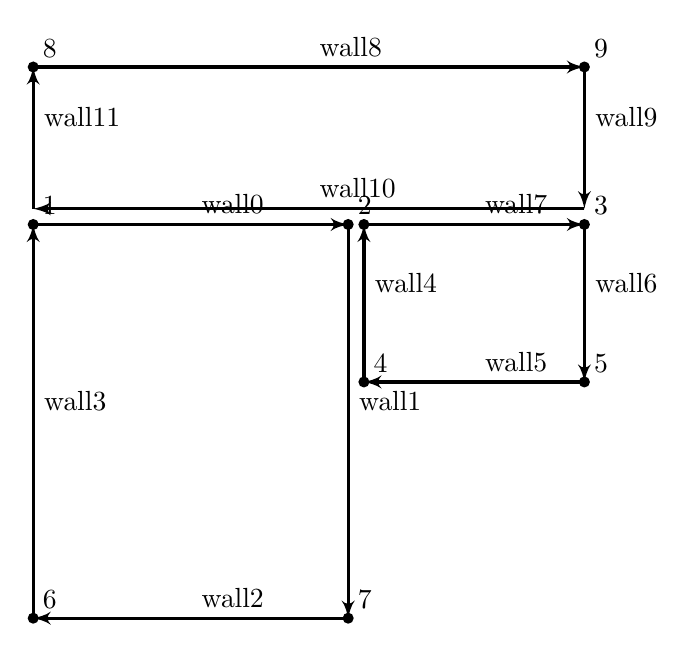
\begin{tikzpicture}[auto,arrow/.style={draw,very thick, -latex'}]
    \coordinate (V1) at (0,0);
    \coordinate (V1a) at (0,0.2);
    \coordinate (V2a) at (4,0);
    \coordinate (V2b) at (4.2,0);
    \coordinate (V3) at (7,0);
    \coordinate (V3a) at (7,0.2);
    \coordinate (V4) at (4.2,-2);
    \coordinate (V5) at (7,-2);
    \coordinate (V6) at (0,-5);
    \coordinate (V7) at (4,-5);

    \coordinate (V8) at (0,2);
    \coordinate (V9) at (7,2);

    % vertices
    \foreach \p/\lbl in {(V1)/1,(V2a)/2,(V2b)/,(V3)/3,(V4)/4,(V5)/5,(V6)/6,(V7)/7,(V8)/8,(V9)/9}
		{
      \fill \p circle (2pt) node[above right] {\lbl};
		}

    % faces		
		\foreach \a/\b/\lbl in {(V1)/(V2a)/wall0,(V2a)/(V7)/wall1,(V7)/(V6)/wall2,(V6)/(V1)/wall3}
		{
		  \draw[arrow] \a -- \b node[midway, color=black,above right] {\lbl};
		}
		\foreach \a/\b/\lbl in {(V4)/(V2b)/wall4,(V5)/(V4)/wall5,(V3)/(V5)/wall6,(V2b)/(V3)/wall7}
		{
		  \draw[arrow] \a -- \b node[midway, color=black,above right] {\lbl};
		}	
		\foreach \a/\b/\lbl in {(V8)/(V9)/wall8,(V9)/(V3a)/wall9,(V3a)/(V1a)/wall10,(V1a)/(V8)/wall11}
		{
		  \draw[arrow] \a -- \b node[midway, color=black,above right] {\lbl};
		}	
		
	\end{tikzpicture}
}
\end{figure}

\newpage

\begin{lstlisting}[language=json,firstnumber=1,basicstyle=\small]
[
	{
    "label": "WALL",
    "attributes": {
      "id" : "wall0",
      "left" : 0,
      "top" : 0,
      "width" : 4000,
      "height" : 2400,
      "origin" : [ 0, 3000, 2400 ],
      "x" : [ 1, 0, 0],
      "y" : [ 0, 0, -1]
    },
    "left": 1,
    "right": 2,
    "crosslink": [ ]
  },
  {
    "label": "WALL",
    "attributes": {
      "id" : "wall1",
      "left" : 0,
      "top" : 0,
      "width" : ...,
      "height" : ...,
      "origin" : ...,
      "x" : ...,
      "y" : ...
    },
    "left": 2,
    "right": 7,
    "crosslink": [ "wall5" ]
  },
	...	
  {
    "label": "DOOR",
    "attributes": {
      "left" : 500,
      "top" : 415,
      "width" : 735,
      "height" : 1985,
      "wallid" : "wall0"
    }
  },	
]
	
\end{lstlisting}

 
\end{document}